\chapter{Background}\label{chap:background}
This Chapter will discuss some background related to the topic of this work. Section \ref{sec:neural_networks} discusses neural networks, while section \ref{sec:adversarial_attacks} introduces both adversarial attacks and defenses. Section \ref{sec:pso} talks about \gls{pso} and some of its improvements over the years.\\

\section{Neural networks}\label{sec:neural_networks}
Ever since the invention of computer systems, it has always been a goal of scientists and engineers to create \gls{ai}. Current state-of-the-art approaches are mimicking the human brain, more specifically the neurons inside the brain. Already in the fifties, Rosenblatt introduced his perceptron \cite{rosenblatt_perceptron_1958}. The perceptron is a single neuron able to learn binary linearly separable patterns. It does so by finding a hyperplane that separates the two classes. This hyperplane is called the decision surface or decision boundary and the perceptron itself is called a classifier. Geometric regions separated by a decision boundary are called decision regions. The concept of linear separability is explained in Figure~\ref{fig:linear_separability} in two dimensions. In Figure~\ref{fig:decision_boundaries_decision_regions}, the decision boundaries and decision regions are explained visually. \\

Unfortunately, not all patterns are linearly separable. To overcome this problem, the neurons can be layered, creating an \gls{ann} in the process. Layering neurons sequentially is essentially a linear combination of neurons. This in itself does not create non-linear decision surfaces. Non-linear activation functions are added for the \gls{ann} to be able to learn more complex decision boundaries. Some commonly used activation functions are \gls{relu} \cite{relu}, Heaviside step function \cite{heaviside} and softmax \cite{softmax} (or sigmoid when used on scalars). In Figure~\ref{fig:activation_functions} the plots of some activation functions can be found.\\ 

\newpage
The neurons can be combined in different ways to create different \gls{ann} architectures. Each architecture has its strengths and weaknesses. \glspl{cnn} excel in classifying visual data \cite{face_recognition_survey, cnn_1, cnn_2}, whilst \glspl{rnn} are widely used when there exist dependencies inside the data, such as in speech recognition \cite{speech_1, speech_2} or time series prediction \cite{time_series_1}. More recent research focuses on \glspl{dnn}, due to the ever-increasing computational power available. \gls{dnn} approaches can compare to and even surpass human performance on very specific tasks \cite{alpha_go_google, imagenet_dnn}.\\ 

Most \glspl{ann} are not built from individual neurons, but rather from layers of neurons. An \gls{ann} architecture describes the different layers of which the network consists. The most basic type of layer is the fully connected or dense layer. This layer, as the name suggests, consists of neurons that are connected to all neurons of the previous layer. Every neuron in this layer outputs a value based on the perceptron rule:
\begin{align*}
	y = b + W \cdot X
\end{align*} 
Here $y$ is the output of the neuron, $b$ is the bias, $W$ is the weight matrix and $X$ is the vector consisting of the outputs of the previous layer. The values of the bias and weights are learned based on the training data. $W \cdot X$ is the dot product $\sum_{i=1}^nw_ix_i$, where $n$ is the number of neurons in the previous layer \cite{perceptron_wikipedia}.\\

Activation layers apply activation functions to their inputs. They can be standalone layers, but more frequently they are integrated into other layers.\\ 

\begin{figure}
\tikzset{every picture/.style={line width=0.75pt}} %set default line width to 0.75pt        
\centering
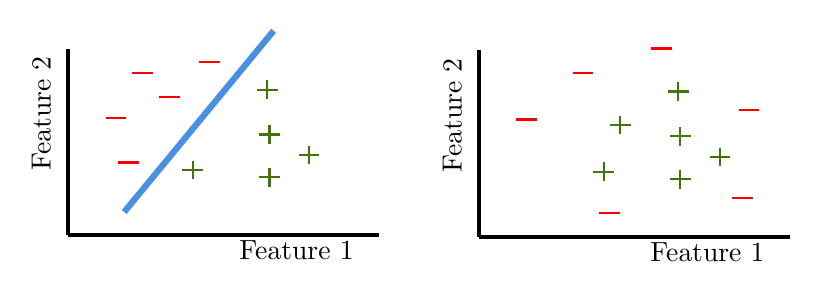
\begin{tikzpicture}[x=0.75pt,y=0.75pt,yscale=-0.9,xscale=1]
%uncomment if require: \path (0,300); %set diagram left start at 0, and has height of 300

%Straight Lines [id:da34928766651876697] 
\draw [line width=1.5]    (40,220) -- (190,220) ;
%Straight Lines [id:da5068123062544778] 
\draw [line width=1.5]    (40,120) -- (40,220) ;
%Straight Lines [id:da02959929373017789] 
\draw [color={rgb, 255:red, 247; green, 0; blue, 0 }  ,draw opacity=1 ]   (71,133) -- (81,133) ;
%Straight Lines [id:da023175201693992564] 
\draw [color={rgb, 255:red, 65; green, 117; blue, 5 }  ,draw opacity=1 ]   (132,166) -- (142,166) ;
%Straight Lines [id:da12599178724449778] 
\draw [color={rgb, 255:red, 65; green, 117; blue, 5 }  ,draw opacity=1 ]   (137,161) -- (137,171) ;

%Straight Lines [id:da014209875608111044] 
\draw [color={rgb, 255:red, 65; green, 117; blue, 5 }  ,draw opacity=1 ]   (95,185) -- (105,185) ;
%Straight Lines [id:da8046955093022794] 
\draw [color={rgb, 255:red, 65; green, 117; blue, 5 }  ,draw opacity=1 ]   (100,180) -- (100,190) ;

%Straight Lines [id:da8257858393303268] 
\draw [color={rgb, 255:red, 65; green, 117; blue, 5 }  ,draw opacity=1 ]   (151,177) -- (161,177) ;
%Straight Lines [id:da9904899777355851] 
\draw [color={rgb, 255:red, 65; green, 117; blue, 5 }  ,draw opacity=1 ]   (156,172) -- (156,182) ;

%Straight Lines [id:da4558392192767111] 
\draw [color={rgb, 255:red, 65; green, 117; blue, 5 }  ,draw opacity=1 ]   (132,189) -- (142,189) ;
%Straight Lines [id:da6277106773918533] 
\draw [color={rgb, 255:red, 65; green, 117; blue, 5 }  ,draw opacity=1 ]   (137,184) -- (137,194) ;

%Straight Lines [id:da6088809310233947] 
\draw [color={rgb, 255:red, 65; green, 117; blue, 5 }  ,draw opacity=1 ]   (131,142) -- (141,142) ;
%Straight Lines [id:da9717175839575936] 
\draw [color={rgb, 255:red, 65; green, 117; blue, 5 }  ,draw opacity=1 ]   (136,137) -- (136,147) ;

%Straight Lines [id:da05579332834233042] 
\draw [color={rgb, 255:red, 247; green, 0; blue, 0 }  ,draw opacity=1 ]   (84,146) -- (94,146) ;
%Straight Lines [id:da9339907902154778] 
\draw [color={rgb, 255:red, 247; green, 0; blue, 0 }  ,draw opacity=1 ]   (64,181) -- (74,181) ;
%Straight Lines [id:da801343700133325] 
\draw [color={rgb, 255:red, 247; green, 0; blue, 0 }  ,draw opacity=1 ]   (103,127) -- (113,127) ;
%Straight Lines [id:da6207217857469742] 
\draw [color={rgb, 255:red, 247; green, 0; blue, 0 }  ,draw opacity=1 ]   (58,157) -- (68,157) ;

%Straight Lines [id:da9774802467048496] 
\draw [line width=1.5]    (238,221) -- (388,221) ;
%Straight Lines [id:da8926029470752344] 
\draw [line width=1.5]    (238,121) -- (238,221) ;
%Straight Lines [id:da391932663930169] 
\draw [color={rgb, 255:red, 247; green, 0; blue, 0 }  ,draw opacity=1 ]   (360,200) -- (370,200) ;
%Straight Lines [id:da45698367355392255] 
\draw [color={rgb, 255:red, 65; green, 117; blue, 5 }  ,draw opacity=1 ]   (330,167) -- (340,167) ;
%Straight Lines [id:da8509197980874896] 
\draw [color={rgb, 255:red, 65; green, 117; blue, 5 }  ,draw opacity=1 ]   (335,162) -- (335,172) ;

%Straight Lines [id:da46487388742354385] 
\draw [color={rgb, 255:red, 65; green, 117; blue, 5 }  ,draw opacity=1 ]   (293,186) -- (303,186) ;
%Straight Lines [id:da6402947556346299] 
\draw [color={rgb, 255:red, 65; green, 117; blue, 5 }  ,draw opacity=1 ]   (298,181) -- (298,191) ;

%Straight Lines [id:da371430190479477] 
\draw [color={rgb, 255:red, 65; green, 117; blue, 5 }  ,draw opacity=1 ]   (349,178) -- (359,178) ;
%Straight Lines [id:da029152498087926304] 
\draw [color={rgb, 255:red, 65; green, 117; blue, 5 }  ,draw opacity=1 ]   (354,173) -- (354,183) ;

%Straight Lines [id:da7641303373625803] 
\draw [color={rgb, 255:red, 65; green, 117; blue, 5 }  ,draw opacity=1 ]   (330,190) -- (340,190) ;
%Straight Lines [id:da8503441823041022] 
\draw [color={rgb, 255:red, 65; green, 117; blue, 5 }  ,draw opacity=1 ]   (335,185) -- (335,195) ;

%Straight Lines [id:da14090483844456858] 
\draw [color={rgb, 255:red, 65; green, 117; blue, 5 }  ,draw opacity=1 ]   (329,143) -- (339,143) ;
%Straight Lines [id:da10211881619757635] 
\draw [color={rgb, 255:red, 65; green, 117; blue, 5 }  ,draw opacity=1 ]   (334,138) -- (334,148) ;

%Straight Lines [id:da8074255152632699] 
\draw [color={rgb, 255:red, 247; green, 0; blue, 0 }  ,draw opacity=1 ]   (296,208) -- (306,208) ;
%Straight Lines [id:da01705778265856206] 
\draw [color={rgb, 255:red, 247; green, 0; blue, 0 }  ,draw opacity=1 ]   (363,153) -- (373,153) ;
%Straight Lines [id:da4845113413868791] 
\draw [color={rgb, 255:red, 247; green, 0; blue, 0 }  ,draw opacity=1 ]   (283,133) -- (293,133) ;
%Straight Lines [id:da861487465385409] 
\draw [color={rgb, 255:red, 247; green, 0; blue, 0 }  ,draw opacity=1 ]   (256,158) -- (266,158) ;
%Straight Lines [id:da9913185077125697] 
\draw [color={rgb, 255:red, 247; green, 0; blue, 0 }  ,draw opacity=1 ]   (321,120) -- (331,120) ;
%Straight Lines [id:da016655837516902583] 
\draw [color={rgb, 255:red, 65; green, 117; blue, 5 }  ,draw opacity=1 ]   (301,161) -- (311,161) ;
%Straight Lines [id:da48554389877316395] 
\draw [color={rgb, 255:red, 65; green, 117; blue, 5 }  ,draw opacity=1 ]   (306,156) -- (306,166) ;


%Straight Lines [id:da7796305041163321] 
\draw [color={rgb, 255:red, 74; green, 144; blue, 226 }  ,draw opacity=1 ][line width=2.25]    (139,110.5) -- (67,207.5) ;

% Text Node
\draw (319,222) node [anchor=north west][inner sep=0.75pt]   [align=left] {Feature 1};
% Text Node
\draw (219,188) node [anchor=north west][inner sep=0.75pt]  [rotate=-270] [align=left] {Feature 2};
% Text Node
\draw (121,221) node [anchor=north west][inner sep=0.75pt]   [align=left] {Feature 1};
% Text Node
\draw (21,187) node [anchor=north west][inner sep=0.75pt]  [rotate=-270] [align=left] {Feature 2};


\end{tikzpicture}
\caption[Linear separability]{Linearly separable classes are on the left and non-linearly separable classes on the right. Two classes are linearly separable if there exists a hyperplane for which all examples of one class are on the same side of this hyperplane, whilst all examples of the other class are on the other side of the hyperplane. In two dimensions, the hyperplane is a straight line.}
\label{fig:linear_separability}
\end{figure}

\begin{figure}
\centering
\tikzset{every picture/.style={line width=0.75pt}} %set default line width to 0.75pt        
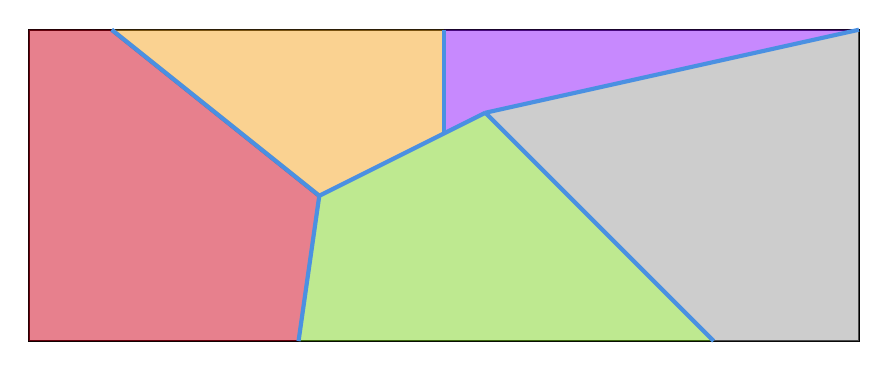
\begin{tikzpicture}[x=0.75pt,y=0.75pt,yscale=-1,xscale=1]
%uncomment if require: \path (0,300); %set diagram left start at 0, and has height of 300

%Shape: Rectangle [id:dp93531352845845] 
\draw   (10,10) -- (410,10) -- (410,160) -- (10,160) -- cycle ;
%Straight Lines [id:da6152066863993235] 
\draw [color={rgb, 255:red, 74; green, 144; blue, 226 }  ,draw opacity=1 ][line width=1.5]    (50,10) -- (150,90) ;
%Shape: Polygon [id:ds7775874145177377] 
\draw  [draw opacity=0][fill={rgb, 255:red, 208; green, 2; blue, 27 }  ,fill opacity=0.5 ] (10,10) -- (50,10) -- (150,90) -- (140,160) -- (10,160) -- cycle ;
%Shape: Polygon [id:ds9784233202991128] 
\draw  [draw opacity=0][fill={rgb, 255:red, 245; green, 166; blue, 35 }  ,fill opacity=0.5 ] (50,10) -- (210,10) -- (210,60) -- (150,90) -- cycle ;
%Straight Lines [id:da46278066568077114] 
\draw [color={rgb, 255:red, 74; green, 144; blue, 226 }  ,draw opacity=1 ][line width=1.5]    (50,10) -- (150,90) ;
%Shape: Polygon [id:ds26003561212820947] 
\draw  [draw opacity=0][fill={rgb, 255:red, 126; green, 211; blue, 33 }  ,fill opacity=0.5 ] (150,90) -- (230,50) -- (340,160) -- (140,160) -- cycle ;
%Shape: Polygon [id:ds9559236222145457] 
\draw  [draw opacity=0][fill={rgb, 255:red, 144; green, 19; blue, 254 }  ,fill opacity=0.5 ] (210,60) -- (230,50) -- (410,10) -- (210,10) -- cycle ;
%Shape: Polygon [id:ds03375440764371551] 
\draw  [draw opacity=0][fill={rgb, 255:red, 155; green, 155; blue, 155 }  ,fill opacity=0.5 ] (230,50) -- (410,10) -- (410,120) -- (410,160) -- (340,160) -- cycle ;
%Straight Lines [id:da4209706928929018] 
\draw [color={rgb, 255:red, 74; green, 144; blue, 226 }  ,draw opacity=1 ][line width=1.5]    (150,90) -- (140,160) ;
%Straight Lines [id:da8034752362025392] 
\draw [color={rgb, 255:red, 74; green, 144; blue, 226 }  ,draw opacity=1 ][line width=1.5]    (150,90) -- (230,50) ;
%Straight Lines [id:da8987706587716273] 
\draw [color={rgb, 255:red, 74; green, 144; blue, 226 }  ,draw opacity=1 ][line width=1.5]    (210,10) -- (210,60) ;
%Straight Lines [id:da07108977100440117] 
\draw [color={rgb, 255:red, 74; green, 144; blue, 226 }  ,draw opacity=1 ][line width=1.5]    (230,50) -- (410,10) ;
%Straight Lines [id:da5244033806754336] 
\draw [color={rgb, 255:red, 74; green, 144; blue, 226 }  ,draw opacity=1 ][line width=1.5]    (230,50) -- (340,160) ;
\end{tikzpicture}
\caption[Decision boundaries and decision regions]{Decision boundaries (blue lines) separate different decision regions (colored regions).}
\label{fig:decision_boundaries_decision_regions}
\end{figure}

\begin{minipage}{\textwidth}
Convolution layers \cite{mnist} are the main building blocks of \glspl{cnn}. Convolution layers map inputs to so-called feature maps. A filter~$W$ slides over the input~$X$ from left to right top to bottom. At every position, the dot product $W\cdot X$ of the frame and the underlying values of the input are computed. This value is placed at the corresponding position of the feature map. Higher values of the dot product (for a fixed value of $\|W\|$) mean that $W$ and $X$ are more similar at this position of $X$. The feature map, therefore, indicates where in the input~$X$ a certain pattern~$W$ can be found. This process is translation-invariant, meaning that a certain pattern can be detected at any location of $X$. Scale and rotation invariance can be achieved by repeating the process for scaled and rotated filters. This invariance is the main reason why \glspl{cnn} are widely used for visual data. An example of a convolution layer is shown in Figure \ref{fig:convolution}.\\
\end{minipage}


\begin{minipage}{\textwidth}
The use of convolution layers tends to cause an explosion in the dimensionality of the data. One filter will produce a feature map that is smaller than the original input. But a convolution layer typically consists of many filters, causing the explosion in the number of connections and weights. Pooling or subsampling layers \cite{mnist} alleviate this problem by aggregating nearby points. The aggregation happens using a sliding window similar to a convolution layer. This approach of reducing dimensionality has the added benefit that the output of the model is less sensitive to the exact location of a pattern. Some frequently used pooling layers are the MaxPooling and AveragePooling layers. They aggregate nearby points using the maximum and average values respectively. Convolution and pooling layers are often used in combination with each other and are repeated multiple times. This allows the \gls{cnn} to detect patterns at different scales.\\
\end{minipage}

 




\begin{figure}
\centering
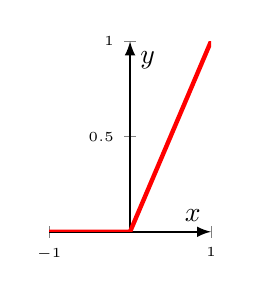
\begin{tikzpicture}
\begin{axis}[width=0.30\textwidth,
height=4cm,
axis lines=middle,
xlabel=$x$,
ylabel=$y$,
xmin=-1,
xmax=1,
ymin=0,
ymax=1,
xtick={-1,1},
ytick={0,0.5,1},
axis line style={-latex},
ticklabel style={font=\tiny,fill=white},
]
\addplot[ultra thick, color=red]{max(0,x)};
\end{axis}
\end{tikzpicture}
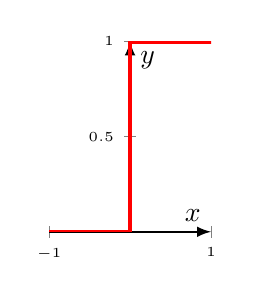
\begin{tikzpicture}
\begin{axis}[width=0.30\textwidth,
height=4cm,
axis lines=middle,
xlabel=$x$,
ylabel=$y$,
xmin=-1,
xmax=1,
ymin=0,
ymax=1,
xtick={-1,1},
ytick={0,0.5,1},
axis line style={-latex},
ticklabel style={font=\tiny,fill=white},
]
\addplot+[const plot, no marks, ultra thick, color=red] coordinates {(-10,0) (0,1) (10, 1)};
\end{axis}
\end{tikzpicture}
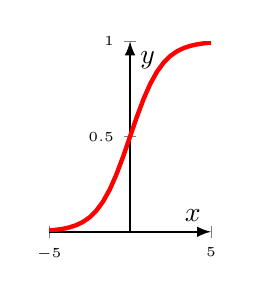
\begin{tikzpicture}
\begin{axis}[width=0.30\textwidth,
height=4cm,
axis lines=middle,
xlabel=$x$,
ylabel=$y$,
xmin=-5,
xmax=5,
ymin=0,
ymax=1,
xtick={-5,5},
ytick={0,0.5,1},
axis line style={-latex},
ticklabel style={font=\tiny,fill=white},
]
\addplot[ultra thick, color=red]{exp(x) / (1 + exp(x))};
\end{axis}
\end{tikzpicture}
\caption[Activiation functions]{Plots of different activation functions. From left to right: \gls{relu}, Heaviside step and sigmoid.}
\label{fig:activation_functions}
\end{figure}

\begin{figure}
\centering
\tikzset{every picture/.style={line width=0.75pt}} %set default line width to 0.75pt        

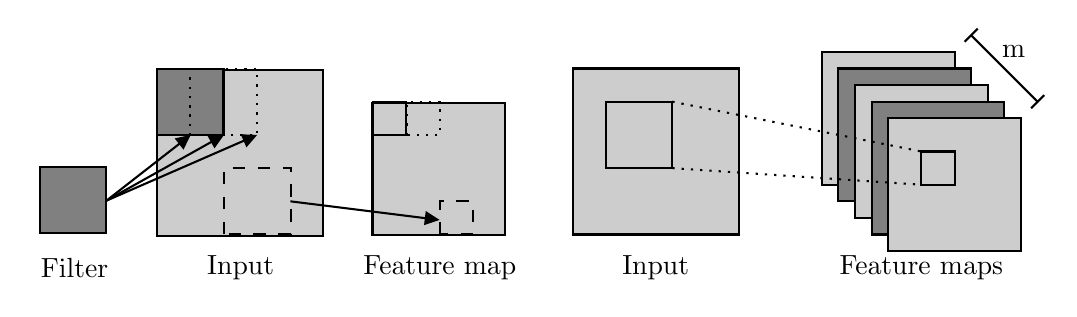
\begin{tikzpicture}[x=0.75pt,y=0.75pt,yscale=-.8,xscale=.8]
%uncomment if require: \path (0,320); %set diagram left start at 0, and has height of 320

%Shape: Rectangle [id:dp16302678045833785] 
\draw  [fill={rgb, 255:red, 128; green, 128; blue, 128 }  ,fill opacity=1 ] (19.22,129.32) -- (19.22,89.32) -- (59.22,89.32) -- (59.22,129.32) -- cycle ;
%Shape: Rectangle [id:dp4740979399382914] 
\draw  [fill={rgb, 255:red, 155; green, 155; blue, 155 }  ,fill opacity=0.5 ] (89.61,130.67) -- (89.61,30.67) -- (189.61,30.67) -- (189.61,130.67) -- cycle ;
%Shape: Rectangle [id:dp758935281388128] 
\draw  [fill={rgb, 255:red, 128; green, 128; blue, 128 }  ,fill opacity=1 ] (89.73,70.27) -- (89.73,30.27) -- (129.73,30.27) -- (129.73,70.27) -- cycle ;
%Shape: Rectangle [id:dp25147604731143414] 
\draw  [dash pattern={on 0.84pt off 2.51pt}][line width=0.75]  (109.73,70.27) -- (109.73,30.27) -- (149.73,30.27) -- (149.73,70.27) -- cycle ;
%Straight Lines [id:da8918779373551835] 
\draw    (59.22,109.59) -- (147.25,71.2) ;
\draw [shift={(150,70)}, rotate = 156.44] [fill={rgb, 255:red, 0; green, 0; blue, 0 }  ][line width=0.08]  [draw opacity=0] (8.93,-4.29) -- (0,0) -- (8.93,4.29) -- cycle    ;
%Straight Lines [id:da6145564233685059] 
\draw    (59.22,109.59) -- (127.38,71.46) ;
\draw [shift={(130,70)}, rotate = 150.78] [fill={rgb, 255:red, 0; green, 0; blue, 0 }  ][line width=0.08]  [draw opacity=0] (8.93,-4.29) -- (0,0) -- (8.93,4.29) -- cycle    ;
%Straight Lines [id:da19666841950671765] 
\draw    (59.22,109.59) -- (107.63,71.84) ;
\draw [shift={(110,70)}, rotate = 142.06] [fill={rgb, 255:red, 0; green, 0; blue, 0 }  ][line width=0.08]  [draw opacity=0] (8.93,-4.29) -- (0,0) -- (8.93,4.29) -- cycle    ;
%Shape: Rectangle [id:dp7649040729081236] 
\draw  [fill={rgb, 255:red, 155; green, 155; blue, 155 }  ,fill opacity=0.5 ] (219.46,130.53) -- (219.46,50.53) -- (299.46,50.53) -- (299.46,130.53) -- cycle ;
%Straight Lines [id:da025473948126214063] 
\draw    (170,110) -- (256.88,120.84) ;
\draw [shift={(259.86,121.21)}, rotate = 187.11] [fill={rgb, 255:red, 0; green, 0; blue, 0 }  ][line width=0.08]  [draw opacity=0] (8.93,-4.29) -- (0,0) -- (8.93,4.29) -- cycle    ;
%Shape: Square [id:dp7289182921794495] 
\draw   (219.86,70.13) -- (219.86,50.13) -- (239.86,50.13) -- (239.86,70.13) -- cycle ;
%Shape: Square [id:dp3517670098930954] 
\draw  [dash pattern={on 0.84pt off 2.51pt}] (240,70) -- (240,50) -- (260,50) -- (260,70) -- cycle ;
%Shape: Square [id:dp0060719107761508795] 
\draw  [dash pattern={on 4.5pt off 4.5pt}] (130.27,129.73) -- (130.27,89.73) -- (170.27,89.73) -- (170.27,129.73) -- cycle ;
%Shape: Square [id:dp7200889456273163] 
\draw  [dash pattern={on 4.5pt off 4.5pt}] (260,130) -- (260,110) -- (280,110) -- (280,130) -- cycle ;
%Shape: Square [id:dp27953712356059635] 
\draw  [fill={rgb, 255:red, 155; green, 155; blue, 155 }  ,fill opacity=0.5 ] (340,30) -- (440,30) -- (440,130) -- (340,130) -- cycle ;
%Shape: Square [id:dp8345536072101358] 
\draw  [fill={rgb, 255:red, 205; green, 205; blue, 205 }  ,fill opacity=1 ] (490,20) -- (570,20) -- (570,100) -- (490,100) -- cycle ;
%Shape: Square [id:dp25056816796659254] 
\draw  [fill={rgb, 255:red, 128; green, 128; blue, 128 }  ,fill opacity=1 ] (500,30) -- (580,30) -- (580,110) -- (500,110) -- cycle ;
%Shape: Square [id:dp2563580070283613] 
\draw  [fill={rgb, 255:red, 205; green, 205; blue, 205 }  ,fill opacity=1 ] (510,40) -- (590,40) -- (590,120) -- (510,120) -- cycle ;
%Shape: Square [id:dp33054308086122974] 
\draw  [fill={rgb, 255:red, 128; green, 128; blue, 128 }  ,fill opacity=1 ] (520,50) -- (600,50) -- (600,130) -- (520,130) -- cycle ;
%Shape: Square [id:dp0968521898422634] 
\draw  [fill={rgb, 255:red, 205; green, 205; blue, 205 }  ,fill opacity=1 ] (530,60) -- (610,60) -- (610,140) -- (530,140) -- cycle ;

%Shape: Square [id:dp4185921090555962] 
\draw   (550,80) -- (570,80) -- (570,100) -- (550,100) -- cycle ;
%Shape: Square [id:dp04075185233144274] 
\draw   (360,50) -- (400,50) -- (400,90) -- (360,90) -- cycle ;
%Straight Lines [id:da45029223803435126] 
\draw  [dash pattern={on 0.84pt off 2.51pt}]  (400,50) -- (550,80) ;
%Straight Lines [id:da34905935844861546] 
\draw  [dash pattern={on 0.84pt off 2.51pt}]  (400,90) -- (550,100) ;
%Straight Lines [id:da4533763369795718] 
\draw    (580,10) -- (620,50) ;
\draw [shift={(620,50)}, rotate = 225] [color={rgb, 255:red, 0; green, 0; blue, 0 }  ][line width=0.75]    (0,5.59) -- (0,-5.59)   ;
\draw [shift={(580,10)}, rotate = 225] [color={rgb, 255:red, 0; green, 0; blue, 0 }  ][line width=0.75]    (0,5.59) -- (0,-5.59)   ;


% Text Node
\draw (40,150) node   [align=left] {\begin{minipage}[lt]{27.2pt}\setlength\topsep{0pt}
\begin{center}
Filter
\end{center}

\end{minipage}};
% Text Node
\draw (140,150) node   [align=left] {\begin{minipage}[lt]{68pt}\setlength\topsep{0pt}
\begin{center}
Input
\end{center}

\end{minipage}};
% Text Node
\draw (260,150) node   [align=left] {\begin{minipage}[lt]{68pt}\setlength\topsep{0pt}
\begin{center}
Feature map
\end{center}

\end{minipage}};
% Text Node
\draw (610,20) node   [align=left] {\begin{minipage}[lt]{13.6pt}\setlength\topsep{0pt}
m
\end{minipage}};
% Text Node
\draw (390,150) node   [align=left] {\begin{minipage}[lt]{68pt}\setlength\topsep{0pt}
\begin{center}
Input
\end{center}

\end{minipage}};
% Text Node
\draw (550,150) node   [align=left] {\begin{minipage}[lt]{81.6pt}\setlength\topsep{0pt}
\begin{center}
Feature maps
\end{center}

\end{minipage}};
\end{tikzpicture}
\caption[Example of a convolution layer]{Example of a convolution layer. The filter slides over the input from left to right top to bottom. At every position, the dot product of the filter and input image is computed. This value is added to the corresponding position of the feature map. This process is repeated for $m$ different filters leading to $m$ feature maps. Inspired by \cite{convolution_source}.}
\label{fig:convolution}
\end{figure}

\section{Adversarial attacks}\label{sec:adversarial_attacks}
The expressiveness of \glspl{ann} is a double-edged sword. It is the cause of the near-human performance on some tasks, but also of some counter-intuitive properties. As studied by Szegedy et al \cite{szegedy2014intriguing}, one of these properties is the presence of discontinuous decision boundaries. This might cause seemingly identical images to be classified differently. They were the first to define adversarial examples as \textit{"imperceptibly small perturbations to a correctly classified input image, so that it is no longer classified correctly"} \cite{szegedy2014intriguing}. This property of \glspl{ann} might not seem important at first glance, but it can be quite worrisome from a security point of view. Malicious users could craft images to bypass face recognition software \cite{face_recognition} or attack the camera of a self-driving car to misclassify traffic signs \cite{traffic_signs}. These images would seem identical to correctly classified images for humans. Other fields where adversarial examples are of interest include malware detection \cite{malware_detection}, natural language processing \cite{adversarial_nlp} and industrial control systems \cite{adversarial_industrial_control_system}. Adversarial attacks are algorithms used to craft such adversarial examples.\\ 

All adversarial attacks are evaluated against a threat model. A threat model is \textit{"a structured representation of all the information that affects the security of an application"} \cite{threat_model}. This information consists of the goals, knowledge and capabilities of the attacker, the accessibility of the model under attack and the costs of (un)successful attacks.\\

\newpage
Most research on adversarial attacks is done using images. Researchers have the most freedom in this domain since a slightly altered image is still an image with roughly the same contents. Slightly modifying an industrial control system, however, might cause complete disruption of the system. All fundamental adversarial research is also performed in the domain of image classification. For this reason, this work focuses on adversarial attacks on images only.\\ 


\subsection{Adversarial attacks terminology}
Adversarial attacks are generally divided into two categories, white-box attacks and black-box attacks. In a white-box attack, the attacker has complete knowledge of the classifier under attack. This knowledge consists of the architecture, parameters and thus their gradients and all output of the classifier. Examples of white-box attacks are the \gls{fgsm} \cite{FGSM} or the Carlini \& Wagner attack \cite{cw_attack}.\\

In black-box attacks, the only piece of information the attacker has access to is the output of the model. Depending on the literature, this output consists of the final decision or class label(s) only (decision-based attack) or the class labels and the corresponding confidence scores (score-based attacks). Black-box attacks are more relevant in real scenarios since most attacks are performed on a third-party \gls{api}. These \glspl{api} generally do not reveal the underlying model.\\

Transfer attacks \cite{transfer_attack} try to overcome this hurdle by creating a surrogate model. This is an undefended model similar to the model under attack. This idea is based on the observation that adversarial perturbations often are transferable to other models than the one they were designed for \cite{FGSM}. Attacks can leverage information (such as gradients) from the surrogate model to breach the black-box model. Due to the transferability of adversarial examples, it is also possible to perform so-called zero-query attacks. Zero-query attacks are performed entirely on the surrogate model and the resulting adversarial example is forwarded to the black-box model.\\

Both white-box and black-box attacks can be divided into targeted and untargeted attacks depending on their goal. In a targeted attack, the goal of the attacker is to create an adversarial example with a specific target class. In an untargeted attack, the target class can be any class. Untargeted variants of attacks generally enjoy much more freedom and are therefore able to craft adversarial examples that are closer to the original. Figure \ref{fig:target_vs_untargeted} visually explains the difference between the two types of attack.

\begin{figure}
\centering
\tikzset{every picture/.style={line width=0.75pt}} %set default line width to 0.75pt        
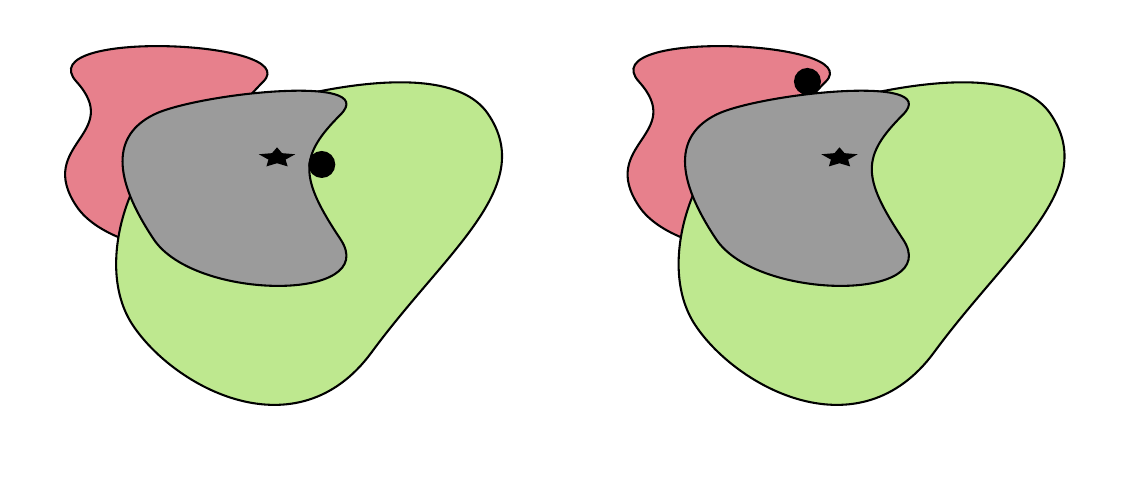
\begin{tikzpicture}[x=0.75pt,y=0.75pt,yscale=-1,xscale=1]
%uncomment if require: \path (0,300); %set diagram left start at 0, and has height of 300

%Shape: Polygon Curved [id:ds8186148148213988] 
\draw  [fill={rgb, 255:red, 231; green, 128; blue, 140 }  ,fill opacity=1 ] (288.8,37.12) .. controls (265.8,11.62) and (398.8,17.12) .. (378.8,37.12) .. controls (358.8,57.12) and (358.8,67.12) .. (378.8,97.12) .. controls (398.8,127.12) and (308.8,127.12) .. (288.8,97.12) .. controls (268.8,67.12) and (311.8,62.62) .. (288.8,37.12) -- cycle ;
%Shape: Polygon Curved [id:ds7649136964229322] 
\draw  [fill={rgb, 255:red, 190; green, 232; blue, 143 }  ,fill opacity=1 ] (337,63.03) .. controls (357,53.03) and (463,17.53) .. (487,52.53) .. controls (511,87.53) and (467,118.53) .. (431,167.53) .. controls (395,216.53) and (336,184.53) .. (316,154.53) .. controls (296,124.53) and (317,73.03) .. (337,63.03) -- cycle ;
%Shape: Polygon Curved [id:ds811213596684691] 
\draw  [fill={rgb, 255:red, 155; green, 155; blue, 155 }  ,fill opacity=1 ] (326,53.03) .. controls (346,43.03) and (436,33.03) .. (416,53.03) .. controls (396,73.03) and (396,83.03) .. (416,113.03) .. controls (436,143.03) and (346,143.03) .. (326,113.03) .. controls (306,83.03) and (306,63.03) .. (326,53.03) -- cycle ;

%Shape: Star [id:dp7949967265036502] 
\draw  [fill={rgb, 255:red, 0; green, 0; blue, 0 }  ,fill opacity=1 ] (385.44,69.53) -- (387.62,72.06) -- (392.51,72.47) -- (388.97,74.44) -- (389.81,77.22) -- (385.44,75.91) -- (381.07,77.22) -- (381.9,74.44) -- (378.36,72.47) -- (383.25,72.06) -- cycle ;

%Shape: Circle [id:dp639830751531604] 
\draw  [fill={rgb, 255:red, 0; green, 0; blue, 0 }  ,fill opacity=1 ] (364,37.03) .. controls (364,33.72) and (366.69,31.03) .. (370,31.03) .. controls (373.31,31.03) and (376,33.72) .. (376,37.03) .. controls (376,40.35) and (373.31,43.03) .. (370,43.03) .. controls (366.69,43.03) and (364,40.35) .. (364,37.03) -- cycle ;
%Shape: Polygon Curved [id:ds526086534908093] 
\draw  [fill={rgb, 255:red, 231; green, 128; blue, 140 }  ,fill opacity=1 ] (17.8,37.12) .. controls (-5.2,11.62) and (127.8,17.12) .. (107.8,37.12) .. controls (87.8,57.12) and (87.8,67.12) .. (107.8,97.12) .. controls (127.8,127.12) and (37.8,127.12) .. (17.8,97.12) .. controls (-2.2,67.12) and (40.8,62.62) .. (17.8,37.12) -- cycle ;
%Shape: Polygon Curved [id:ds40487542108345687] 
\draw  [fill={rgb, 255:red, 190; green, 232; blue, 143 }  ,fill opacity=1 ] (66,63.03) .. controls (86,53.03) and (192,17.53) .. (216,52.53) .. controls (240,87.53) and (196,118.53) .. (160,167.53) .. controls (124,216.53) and (65,184.53) .. (45,154.53) .. controls (25,124.53) and (46,73.03) .. (66,63.03) -- cycle ;
%Shape: Polygon Curved [id:ds8878674517678289] 
\draw  [fill={rgb, 255:red, 155; green, 155; blue, 155 }  ,fill opacity=1 ] (55,53.03) .. controls (75,43.03) and (165,33.03) .. (145,53.03) .. controls (125,73.03) and (125,83.03) .. (145,113.03) .. controls (165,143.03) and (75,143.03) .. (55,113.03) .. controls (35,83.03) and (35,63.03) .. (55,53.03) -- cycle ;

%Shape: Star [id:dp9101553466481458] 
\draw  [fill={rgb, 255:red, 0; green, 0; blue, 0 }  ,fill opacity=1 ] (114.44,69.53) -- (116.62,72.06) -- (121.51,72.47) -- (117.97,74.44) -- (118.81,77.22) -- (114.44,75.91) -- (110.07,77.22) -- (110.9,74.44) -- (107.36,72.47) -- (112.25,72.06) -- cycle ;

%Shape: Circle [id:dp29014472584929707] 
\draw  [fill={rgb, 255:red, 0; green, 0; blue, 0 }  ,fill opacity=1 ] (130,77.03) .. controls (130,73.72) and (132.69,71.03) .. (136,71.03) .. controls (139.31,71.03) and (142,73.72) .. (142,77.03) .. controls (142,80.35) and (139.31,83.03) .. (136,83.03) .. controls (132.69,83.03) and (130,80.35) .. (130,77.03) -- cycle ;
\end{tikzpicture}
\caption[Difference targeted and untargeted attack]{Different decision regions are shown in different colors. An adversarial example is being created starting from the original image (black star). On the left, an untargeted attack is performed. The adversarial example is the image closest to the original image, which is classified differently (black circle). On the right, a targeted attack is performed with the red decision region being the target class. The adversarial example is the image closest to the original image that is in the red decision region.}
\label{fig:target_vs_untargeted}
\end{figure}

What does it mean for images to be close to each other? This is easy to visualize in two dimensions as in Figure \ref{fig:target_vs_untargeted}, but in higher dimensions, this is more difficult. Images reside in $d$-dimensional space, where $d$ is the number of pixels of the image\footnote{For color images in RGB-space, there are actually three times the amount of pixels. A complete set for each color channel.}. Two commonly used distances in higher dimensions are the $L_2$-distance and the $L_\infty$-distance. They are defined as follows:

\begin{align*}
L_2(X, Y) &= \sqrt{\sum_{i=1}^d|x_i - y_i|^2} \\
L_\infty(X, Y) &= \lim_{p\rightarrow \infty}\left( \sum_{i=1}^d|x_i-y_i|^p\right)^{1/p} \\
&= \max (|x_1 - y_1|, |x_2-y_2|, \ldots, |x_d-y_d|)
\end{align*}

In both distances $X$ and $Y$ represent the images and $(x_1, x_2, \ldots, x_i, \ldots, x_d)$ and $(y_1, y_2, \ldots, y_i, \ldots, y_d)$ are the pixel values of $X$ and $Y$ respectively. The $L_2$-distance is also known as the Euclidean distance, which is a generalization of the Pythagorean theorem in more than two dimensions. It takes the pairwise distances between all pixels into account. The $L_\infty$-distance is also called the Chebyshev distance. This distance only depends on the maximal pairwise distance between the two images. By minimizing the $L_\infty$-distance, the maximal pixel-wise difference is minimized \cite{wiki_distances}.  Sometimes the norm notation $\| \cdot \|$ is used instead of the distance notation. A distance is induced by a norm by $d(X,Y) = \| X -Y\|$. The other direction, a distance inducing a norm, is not as trivial. For a distance to induce a norm, the distance has to satisfy the following condition: $d(\alpha X,\alpha Y) = |\alpha | d(X,Y)$. This condition is satisfied in most commonly used distances, but this is not always the case. The discrete distance \cite{discrete_distance} is an example of such a distance and is defined as follows:
\begin{align*}
d(X,Y) = 
\begin{cases}
1, &\text{if } X \neq Y\\
0, &\text{else}
\end{cases}
\end{align*}
Multiplying both $X$ and $Y$ with a fixed value $\alpha$ does not change the outcome of the distance function.\\

\subsection{Adversarial defenses}\label{sec:adversarial_defenses}
The existence of adversarial attacks naturally gave rise to adversarial defenses. These defenses can be categorized based on their objective. They can be either proactive or reactive. The goal of a proactive defense consists of making the models under attack more robust, while reactive defenses aim to identify attacks before they reach the model \cite{adversarial_defense_survey}. Different defensive countermeasures can be taken in each category. The remainder of this section will discuss some commonly used techniques \cite{defenses_survey}.\\

\textbf{Gradient masking} techniques hinder optimization-based attacks by having gradients "\textit{that are not useful}" \cite{not_useful_gradients}. They are also sometimes referred to as obfuscated gradients \cite{obfuscated_gradients}. Three types of obfuscated gradients can be identified. Shattered gradients introduce incorrect or non-existent gradients. Stochastic gradients are caused by random effects in the defense and exploding or vanishing gradients are primarily caused by chaining neural network evaluations. Besides intentionally introducing gradient masking in neural networks, they can also be introduced unintentionally due to the design of the network.\\

\textbf{Defensive distillation}  \cite{defensive_distillation} is a technique that can be classified as gradient masking. The goal of defensive distillation is to smooth the gradients of the model, making it more resilient to small input perturbations. The distillation procedure is done in two steps. First, the model is trained on the original data and labels. This step produces a probabilistic output for each input due to the softmax activation function. Then the network is retrained using the original data and the probabilistic outputs as labels. The probabilistic labels contain additional knowledge that can be exploited to increase the generalizability of the model.\\

\textbf{Adversarial training} \cite{FGSM} techniques inject adversarial examples into the training dataset and retrain the model to create a more resilient model. This is essentially a brute force method to correctly classify some adversarial examples. However, this new model is still susceptible to new adversarial attacks since the decision boundary has only been moved slightly. This can be seen in Figure \ref{fig:adversarial_training}. Adversarial training is however still the most effective method to make models more robust. The technique can be seen as a min-max problem, where the classification loss $L$ has to be minimized against an adversary trying to maximize this same loss \cite{huang}. This problem can be expressed as:

\begin{equation*}
\min_\theta \mathbb{E}_{(x,y) \sim \mathcal{D}} \left[  \max_{\delta \in B(x,\epsilon)} L(\theta,x+\delta,y)\right]
\end{equation*}

An adversary tries to maximize the loss $L$ by adding a perturbation $\delta$ from the allowed set of perturbation $B$ to the original image $x$. Existing attack algorithms can be utilized to maximize the inner part of this problem. This allows the training procedure to minimize the expected loss over the training samples $(x,y)$ of the training distribution $\mathcal{D}$. Maximizing the inner part of the equation corresponds to finding the worst-case examples for a specific model with parameters $\theta$. \gls{fgsm} \cite{FGSM} generates such adversarial examples using the following formula:

\begin{equation*}
x + \epsilon \sgn(\nabla_xL(\theta,x,y))
\end{equation*}

A perturbation is added to the original image $x$ based on the gradient of the loss function $L$. \gls{pgd} \cite{pgd} has been proposed as a more powerful multi-step technique to generate the adversarial examples:

\begin{equation*}
x^{t+1} = \prod_{x+B(x,\epsilon)} (x^t + \alpha \sgn(\nabla_xL(\theta,x,y)))
\end{equation*}

After the generation of adversarial examples, the minimization part of the problem, i.e. the training itself can take place. This approach of generating adversarial examples improved the robustness against adversarial attacks. Today, it is still seen as the way to perform adversarial training in practice \cite{adversarial_training}.\\ 

\textbf{Preprocessing techniques} work on the inputs of a model. Different preprocessing techniques, such as denoising \cite{denoising}, dimensionality reduction \cite{dimensionality_reduction} and image transformations \cite{image_transformations} can be used to defend the model under attack. The goal of all techniques boils down to giving the attacker less control over the exact input that is being fed to the model.\\

Some defenses rely on \textbf{proximity measurements} between the input and the model. An example of this countermeasure is \gls{dknn} by Papernot and McDaniel \cite{dknn}. \gls{dknn} computes support for a decision from a network based on a nearest neighbors search in the training data. Another example is region-based classification \cite{region-based_classification}, where a prediction is made for a given input based on the proximity of training examples.\\ 

\begin{figure}
\centering

\tikzset{every picture/.style={line width=0.75pt}} %set default line width to 0.75pt        

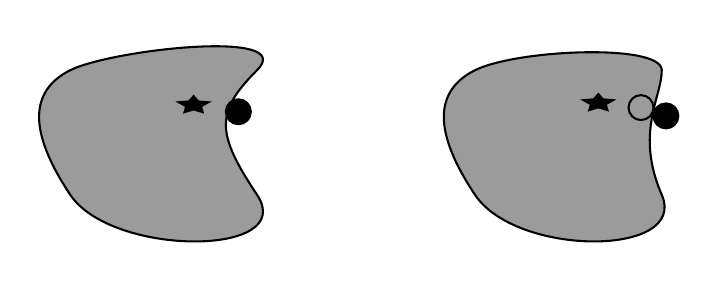
\begin{tikzpicture}[x=0.75pt,y=0.75pt,yscale=-1,xscale=1]
%uncomment if require: \path (0,300); %set diagram left start at 0, and has height of 300

%Shape: Polygon Curved [id:ds8779908352046051] 
\draw  [fill={rgb, 255:red, 155; green, 155; blue, 155 }  ,fill opacity=1 ] (55,57.03) .. controls (75,47.03) and (165,37.03) .. (145,57.03) .. controls (125,77.03) and (125,87.03) .. (145,117.03) .. controls (165,147.03) and (75,147.03) .. (55,117.03) .. controls (35,87.03) and (35,67.03) .. (55,57.03) -- cycle ;
%Shape: Star [id:dp10110664534314551] 
\draw  [fill={rgb, 255:red, 0; green, 0; blue, 0 }  ,fill opacity=1 ] (114.44,69.53) -- (116.62,72.06) -- (121.51,72.47) -- (117.97,74.44) -- (118.81,77.22) -- (114.44,75.91) -- (110.07,77.22) -- (110.9,74.44) -- (107.36,72.47) -- (112.25,72.06) -- cycle ;
%Shape: Circle [id:dp6094270387234269] 
\draw  [fill={rgb, 255:red, 0; green, 0; blue, 0 }  ,fill opacity=1 ] (130,77.03) .. controls (130,73.72) and (132.69,71.03) .. (136,71.03) .. controls (139.31,71.03) and (142,73.72) .. (142,77.03) .. controls (142,80.35) and (139.31,83.03) .. (136,83.03) .. controls (132.69,83.03) and (130,80.35) .. (130,77.03) -- cycle ;
%Shape: Polygon Curved [id:ds9355803976339294] 
\draw  [fill={rgb, 255:red, 155; green, 155; blue, 155 }  ,fill opacity=1 ] (250,57.03) .. controls (270,47.03) and (340,44) .. (340,57.03) .. controls (340,70.07) and (327,87.07) .. (340,117.03) .. controls (353,147) and (270,147.03) .. (250,117.03) .. controls (230,87.03) and (230,67.03) .. (250,57.03) -- cycle ;
%Shape: Star [id:dp952475231363908] 
\draw  [fill={rgb, 255:red, 0; green, 0; blue, 0 }  ,fill opacity=1 ] (309.44,68.53) -- (311.62,71.06) -- (316.51,71.47) -- (312.97,73.44) -- (313.81,76.22) -- (309.44,74.91) -- (305.07,76.22) -- (305.9,73.44) -- (302.36,71.47) -- (307.25,71.06) -- cycle ;
%Shape: Circle [id:dp489720270519854] 
\draw   (324,75.03) .. controls (324,71.72) and (326.69,69.03) .. (330,69.03) .. controls (333.31,69.03) and (336,71.72) .. (336,75.03) .. controls (336,78.35) and (333.31,81.03) .. (330,81.03) .. controls (326.69,81.03) and (324,78.35) .. (324,75.03) -- cycle ;
%Shape: Circle [id:dp014656790375494388] 
\draw  [fill={rgb, 255:red, 0; green, 0; blue, 0 }  ,fill opacity=1 ] (336,79.03) .. controls (336,75.72) and (338.69,73.03) .. (342,73.03) .. controls (345.31,73.03) and (348,75.72) .. (348,79.03) .. controls (348,82.35) and (345.31,85.03) .. (342,85.03) .. controls (338.69,85.03) and (336,82.35) .. (336,79.03) -- cycle ;
\end{tikzpicture}
\caption[Adversarial training]{Decision boundaries before (left) and after (right) adversarial training. Before adversarial training, an adversarial example can be created (black circle). This example is added to the training set and the network is retrained. A new decision surface is created in the process. This surface classifies the previous adversarial example correctly (empty circle), but there is a new opportunity for an adversarial attack (black circle).}
\label{fig:adversarial_training}
\end{figure}


\section{Particle swarm optimization}\label{sec:pso}
\gls{pso} \cite{pso} is an optimization framework part of the \gls{ea} family. In \glspl{ea}, populations of candidate solutions evolve based on mechanisms inspired by the field of biology, such as ant colonies \cite{aco}, mutation and recombination \cite{genetic_algorithm}. The mechanism that inspired \gls{pso} is the behavior of the flocks of birds. The framework has been applied to numerous problems such as routing problems \cite{ev_transport, freight_transport}, diagnosing diseases from imaging \cite{leukemia_pso} and calculating heat transfer coefficients \cite{heat_transfer_pso}.\\

\gls{pso} is a good fit for decision-based adversarial attacks due to the low requirements. It only requires a fitness function defined for positions in the search space. No gradients are needed as opposed to optimization techniques such as gradient descent \cite{gradient_descent}. These gradients are also not available in black-box settings, causing \gls{pso} to be useful in both white- and black-box settings. The multiple starting positions of \gls{pso} can also improve both the efficiency and evasiveness of adversarial attacks as will be shown in section \ref{sec:combining_pso_bba}.\\

In \gls{pso}, different particles~$x$ move through the search space based on a set of rules. Their new position~$x_t$ is determined by their previous position~$x_{t-1}$ and a velocity $v_t$. The velocity depends on the distance to the best position of the swarm~$g$ and the best-known position of the particle~$p$. The distances can be weighted by acceleration coefficients~$c$ to put more emphasis on exploration or exploitation. These values are multiplied by random parameters~$r$ uniformly distributed in~$[0,1]$. The velocity is also dependent on the previous velocity with a corresponding weight~$w$. The best position is determined using a fitness function. This function states how 'fit' or good a certain position is concerning the goal of the optimization problem. Equations~\ref{eq:velocity_update} and \ref{eq:position_update} correspond to the update rules. Each particle $i$ has its own position~$x_{t,i}$ and velocity~$v_{t,i}$ at time step~$t$, but the $i$~index has been omitted for readability. In Figure~\ref{fig:pso}, the steps are graphically represented for a single particle.

\begin{figure}
\centering
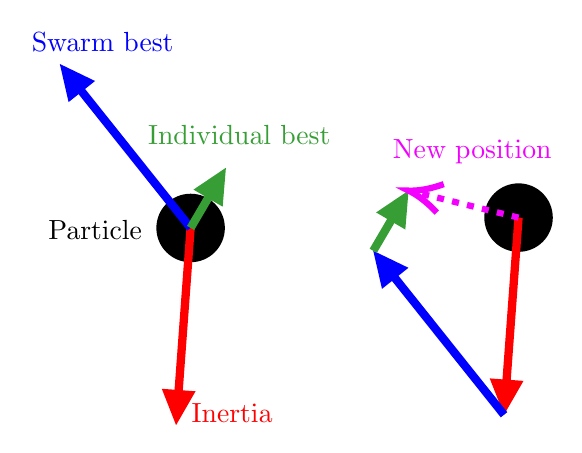
\begin{tikzpicture}[x=0.75pt,y=0.75pt,yscale=-1,xscale=1]

%uncomment if require: \path (0,300); %set diagram left start at 0, and has height of 300

%Shape: Circle [id:dp06935534605548432] 
\draw  [fill={rgb, 255:red, 0; green, 0; blue, 0 }  ,fill opacity=1 ] (100,161) .. controls (100,152.16) and (107.16,145) .. (116,145) .. controls (124.84,145) and (132,152.16) .. (132,161) .. controls (132,169.84) and (124.84,177) .. (116,177) .. controls (107.16,177) and (100,169.84) .. (100,161) -- cycle ;
%Straight Lines [id:da36297070749556615] 
\draw [color={rgb, 255:red, 255; green, 0; blue, 0 }  ,draw opacity=1 ][line width=3]    (116,161) -- (109.44,250.02) ;
\draw [shift={(109,256)}, rotate = 274.21] [fill={rgb, 255:red, 255; green, 0; blue, 0 }  ,fill opacity=1 ][line width=0.08]  [draw opacity=0] (16.97,-8.15) -- (0,0) -- (16.97,8.15) -- cycle    ;
%Shape: Circle [id:dp2975589876543052] 
\draw  [fill={rgb, 255:red, 0; green, 0; blue, 0 }  ,fill opacity=1 ] (258,156) .. controls (258,147.16) and (265.16,140) .. (274,140) .. controls (282.84,140) and (290,147.16) .. (290,156) .. controls (290,164.84) and (282.84,172) .. (274,172) .. controls (265.16,172) and (258,164.84) .. (258,156) -- cycle ;
%Straight Lines [id:da11974704599725938] 
\draw [color={rgb, 255:red, 255; green, 0; blue, 0 }  ,draw opacity=1 ][line width=3]    (274,156) -- (267.44,245.02) ;
\draw [shift={(267,251)}, rotate = 274.21] [fill={rgb, 255:red, 255; green, 0; blue, 0 }  ,fill opacity=1 ][line width=0.08]  [draw opacity=0] (16.97,-8.15) -- (0,0) -- (16.97,8.15) -- cycle    ;
%Straight Lines [id:da34669530870861953] 
\draw [color={rgb, 255:red, 0; green, 0; blue, 255 }  ,draw opacity=1 ][line width=3]    (267,251) -- (207.74,176.69) ;
\draw [shift={(204,172)}, rotate = 51.43] [fill={rgb, 255:red, 0; green, 0; blue, 255 }  ,fill opacity=1 ][line width=0.08]  [draw opacity=0] (16.97,-8.15) -- (0,0) -- (16.97,8.15) -- cycle    ;
%Straight Lines [id:da2944239439562262] 
\draw [color={rgb, 255:red, 55; green, 158; blue, 54 }  ,draw opacity=1 ][line width=3]    (204,172) -- (217.97,148.18) ;
\draw [shift={(221,143)}, rotate = 120.38] [fill={rgb, 255:red, 55; green, 158; blue, 54 }  ,fill opacity=1 ][line width=0.08]  [draw opacity=0] (16.97,-8.15) -- (0,0) -- (16.97,8.15) -- cycle    ;
%Straight Lines [id:da9472051718664152] 
\draw [color={rgb, 255:red, 243; green, 0; blue, 255 }  ,draw opacity=1 ][line width=2.25]  [dash pattern={on 2.53pt off 3.02pt}]  (274,156) -- (224.88,143.95) ;
\draw [shift={(221,143)}, rotate = 13.78] [color={rgb, 255:red, 243; green, 0; blue, 255 }  ,draw opacity=1 ][line width=2.25]    (15.74,-7.06) .. controls (10.01,-3.31) and (4.76,-0.96) .. (0,0) .. controls (4.76,0.96) and (10.01,3.31) .. (15.74,7.06)   ;
%Straight Lines [id:da8503925276289086] 
\draw [color={rgb, 255:red, 0; green, 0; blue, 255 }  ,draw opacity=1 ][line width=3]    (116,161) -- (56.74,86.69) ;
\draw [shift={(53,82)}, rotate = 51.43] [fill={rgb, 255:red, 0; green, 0; blue, 255 }  ,fill opacity=1 ][line width=0.08]  [draw opacity=0] (16.97,-8.15) -- (0,0) -- (16.97,8.15) -- cycle    ;
%Straight Lines [id:da10251717157021911] 
\draw [color={rgb, 255:red, 55; green, 158; blue, 54 }  ,draw opacity=1 ][line width=3]    (116,161) -- (129.97,137.18) ;
\draw [shift={(133,132)}, rotate = 120.38] [fill={rgb, 255:red, 55; green, 158; blue, 54 }  ,fill opacity=1 ][line width=0.08]  [draw opacity=0] (16.97,-8.15) -- (0,0) -- (16.97,8.15) -- cycle    ;

% Text Node
\draw (46,156) node [anchor=north west][inner sep=0.75pt]   [align=left] {Particle};
% Text Node
\draw (115,244) node [anchor=north west][inner sep=0.75pt]   [align=left] {\textcolor[rgb]{1,0,0}{Inertia}};
% Text Node
\draw (38,65) node [anchor=north west][inner sep=0.75pt]  [color={rgb, 255:red, 0; green, 0; blue, 255 }  ,opacity=1 ] [align=left] {Swarm best};
% Text Node
\draw (94,110) node [anchor=north west][inner sep=0.75pt]  [color={rgb, 255:red, 55; green, 158; blue, 54 }  ,opacity=1 ] [align=left] {Individual best};
% Text Node
\draw (212,117) node [anchor=north west][inner sep=0.75pt]   [align=left] {\textcolor[rgb]{0.95,0,1}{New position}};


\end{tikzpicture}
\caption[Particle swarm optimization]{Particles move based on a step towards their best-known position, the swarm's best-known position and a step in the direction of the movement of the previous iteration. The different steps are combined to determine the new position of the particle.}
\label{fig:pso}
\end{figure}

%In \gls{pso}, different particles move through the search space based on a set of rules. Each position in the search space has a given fitness value. This value determines how 'fit' or good a certain position is with respect to the goal of the optimization problem. Every iteration, all particles take a step towards their personal best position, towards the group or swarm's best position and a step in the current direction (inertia). The different step sizes can be weighted depending on the problem at hand. In Figure~\ref{fig:pso}, the steps are graphically represented for a single particle.

\begin{align} 
v_{t} &= \underbrace{wv_{t-1}}_\text{Inertia} + \underbrace{c_pr_p(p_{t-1} - x_{t-1})}_\text{Individual best} + \underbrace{c_gr_g(g_{t-1} - x_{t-1})}_\text{Swarm best} \label{eq:velocity_update}\\
x_{t} &= x_{t-1} + v_{t} \label{eq:position_update}
\end{align}

Ever since the first mention of \gls{pso} in 1995, efforts have been made to improve the framework. The rest of this section will discuss some improvements.\\

The first version of \gls{pso} used a fixed value for the inertia weight $w$. Later it has empirically been shown that a linearly decaying weight improves performance \cite{pso_study}. This allows the algorithm to focus on exploration in the early iterations while shifting its focus to exploitation later on. The rate of decay depends on the high start value~$w_{start}$, the lower end value~$w_{end}$ and the maximum number of iterations $t_{max}$. The weight in iteration~$t$ is calculated as follows:

\begin{align}
w_t = w_{end} + (w_{start} - w_{end})\left(1 - \frac{t}{t_{max}}\right) \label{eq:weight}
\end{align}

In a large search space, particles can be far apart, which can cause the velocities to explode. By limiting the value of velocities to $v_{max}$, the swarm can be stabilized and the probability of finding an optimum is increased \cite{pso}.\\

Clerc and Kennedy \cite{constriction_factor} studied \gls{pso} from a dynamic systems point of view. They provided a theoretically backed solution to the problem of the exploding velocities. Instead of limiting the value of the velocity, something of which only empirical evidence has been given, they proposed the use of a constriction factor $\chi$. The constriction factor can prevent the velocity explosion, whilst avoiding premature convergence to local optima. The velocity update of equation \ref{eq:velocity_update} is altered as follows:
\begin{align*}
	v_{t} &= \chi (v_{t-1} + c_pr_p(p_{t-1} - x_{t-1}) + c_gr_g(g_{t-1} - x_{t-1}))
\end{align*}

\newpage
The inertia weight $w$ is dropped and the entire sum is multiplied by $\chi$. The value of $\chi$ is calculated as follows:
\begin{align*}
	\chi = 
	\begin{cases}
		\sqrt{\frac{2\kappa}{C-2+\sqrt{C^2-4C}}}, &C>4\\
		\sqrt{\kappa}, 							&\text{else}
	\end{cases}
\end{align*}
Here $C$ is the sum of the acceleration coefficients $c_p$ and $c_g$ and $\kappa$ is a user-defined value to determine the rate of convergence. Increasing $\kappa$ slows down convergence, but causes a more thorough search to take place. The value of $\kappa$ should be contained in the interval $]0, 1[$.\\ 

Another improvement on vanilla\footnote{Vanilla is used to refer to software or algorithms not altered from their original form \cite{vanilla}.} \gls{pso} is \gls{mgrr} \gls{pso} \cite{opposite_cs}. The swarm is split into two groups with opposite acceleration coefficients. The first group, with a larger $c_p$, is more attracted to the local optima, while the second group, with a larger $c_g$, moves to the global optimum. The combination of the two groups accounts for more variation during the search process. This in turn aids in the convergence to the global optimum.\\ 

Even with the multi-group improvement, the particles can get trapped in local optima, as is the case in vanilla \gls{pso}. Whenever the swarm is stuck in a local optimum, half of the particles are randomly redistributed. The particles that will be redistributed will change approximately half of their values. The redistribution gives the algorithm a chance to escape the local optimum.\\
 
Experimental results show that \gls{mgrr}-\gls{pso} has better performance than the vanilla variant \cite{opposite_cs}. The convergence is also faster and less dependent on the starting positions of the particles. Even the variant without the random redistribution outperforms vanilla \gls{pso}.\\  

\begin{minipage}{\textwidth}
\gls{pso} is often combined with other algorithms in so-called hybridization techniques. The goal of this combination is to create an algorithm that contains the beneficial properties of both its constituents. Some commonly used algorithms combined with \gls{pso} are genetic algorithms \cite{genetic_algorithm}, differential evolution \cite{differential_evolution} and ant colony optimization \cite{aco}. Hybridization is most commonly done in three different ways. In a first way, one algorithm is used before the other. The first algorithm performs optimization on the population used in the second algorithm. The second way divides the entire population into two groups and every group is optimized with a constituent algorithm. Some inter-group communication is required for this approach to work. The idea behind this technique is similar to the \gls{mgrr} approach discussed earlier. The third way incorporates specific parts of an algorithm as a local search operator in the other. Thangaraj et al. \cite{hybridization_survey} studied 64 hybridization algorithms containing \gls{pso} as one of the constituents. They found that the combination of differential evolution and \gls{pso} edges out the other hybrid approaches in terms of average error. However, all techniques outperform vanilla \gls{pso} using the error metric.\\
\end{minipage}


Another approach to prevent the particles of the swarm to converge to local optima is to restrict the communication inside the swarm. In vanilla \gls{pso} all particles know the best position of the entire swarm. All particles will take a step towards this position in the next iteration of the algorithm. This causes the particles to converge to each other and limits the exploration of the search space. To restrict this knowledge, different communication topologies can be used. Some topologies are depicted in Figure \ref{fig:pso_topologies}. Here the nodes represent the different particles and the edges show the possibility of communication between these particles. The fully connected topology is the standard topology used in \gls{pso}. A ring topology limits communication of the best position to two neighbors per particle. The pyramid topology is similar to the ring topology, but there exists one particle that can communicate with all other particles. Neighbors in the topologies can be determined based on pre-defined indices or the position of the particles in search space. The latter requires more computations. It has been shown that the best topology is highly problem dependent and that the size of the swarm plays a significant role in the choice of the best topology \cite{pso_topologies}. Combinations between the fully connected and ring topology are also possible and show promising results \cite{fc_ring}.



\begin{figure}
	\centering
	\subfloat[Fully connected] {%
	\label{fig:fully_connected}%
	\begin{tikzpicture}[y=0.3\linewidth]
		\path
    node[
      regular polygon,
      regular polygon sides=6,
      draw,
      inner sep=.7cm,
    ] (hexagon) {}
    %
    % Annotations
    (hexagon.corner 1) node[above] {}
    (hexagon.corner 2) node[above] {}
    (hexagon.corner 3) node[left] {}
    (hexagon.corner 4) node[below] {}
    (hexagon.corner 5) node[below] {}
    (hexagon.corner 6) node[right] {}
    %
    % Small filled black circles
    plot[
      mark=*,
      samples at={1, ..., 6},
    ] (hexagon.corner \x)
  ;
  \draw (hexagon.corner 1) -- (hexagon.corner 3);
  \draw (hexagon.corner 1) -- (hexagon.corner 4);
  \draw (hexagon.corner 1) -- (hexagon.corner 5);
  \draw (hexagon.corner 2) -- (hexagon.corner 4);
  \draw (hexagon.corner 2) -- (hexagon.corner 5);
  \draw (hexagon.corner 2) -- (hexagon.corner 6);
  \draw (hexagon.corner 3) -- (hexagon.corner 5);
  \draw (hexagon.corner 3) -- (hexagon.corner 6);
  \draw (hexagon.corner 4) -- (hexagon.corner 6);
	\end{tikzpicture}
	} \quad
	\subfloat[Ring] {%
	\label{fig:ring}%
	\begin{tikzpicture}[y=0.3\linewidth]
	\path
    node[
      regular polygon,
      regular polygon sides=6,
      draw,
      inner sep=.7cm,
    ] (hexagon) {}
    %
    % Annotations
    (hexagon.corner 1) node[above] {}
    (hexagon.corner 2) node[above] {}
    (hexagon.corner 3) node[left] {}
    (hexagon.corner 4) node[below] {}
    (hexagon.corner 5) node[below] {}
    (hexagon.corner 6) node[right] {}
    %
    % Small filled black circles
    plot[
      mark=*,
      samples at={1, ..., 6},
    ] (hexagon.corner \x)
  ;
	\end{tikzpicture}
	} \quad
	\subfloat[Pyramid] {%
	\label{fig:pyramid}%
	\begin{tikzpicture}[y=0.3\linewidth]
	\path
    node[
      regular polygon,
      regular polygon sides=5,
      draw,
      inner sep=.7cm,
    ] (hexagon) {}
    %
    % Annotations
    (hexagon.corner 1) node[above] {}
    (hexagon.corner 2) node[above] {}
    (hexagon.corner 3) node[left] {}
    (hexagon.corner 4) node[below] {}
    (hexagon.corner 5) node[below] {}
    %
    % Small filled black circles
    plot[
      mark=*,
      samples at={1, ..., 5},
    ] (hexagon.corner \x)
  	plot[
      mark=*,
    ] (0,0)
  ;
  
  \draw (0,0) -- (hexagon.corner 1);
  \draw (0,0) -- (hexagon.corner 2);
  \draw (0,0) -- (hexagon.corner 3);
  \draw (0,0) -- (hexagon.corner 4);
  \draw (0,0) -- (hexagon.corner 5);
	\end{tikzpicture}
	}
	\caption[PSO communication topologies]{Different communication topologies for the \gls{pso} framework. The particles are represented by the nodes and the edges represent the communication channels. Inspired by \cite{pso_topologies}.}
	\label{fig:pso_topologies}
\end{figure}
